% -*- ispell-dictionary: "russian" -*-
% \documentclass[12pt,a4paper]{memoir}
\documentclass[12pt,a4paper]{ltxdoc}
\usepackage{unicode-math}
\usepackage{luatextra}
\defaultfontfeatures{Renderer=Basic, Ligatures=TeX}
\usepackage{ifxetex}
\usepackage{ifluatex}
\usepackage{graphicx}
%\usepackage[english,russian]{babel}
\usepackage{polyglossia}
\usepackage{hyperref}
\usepackage[a4paper, tmargin=1in,bmargin=1in,lmargin=1in,rmargin=1in]{geometry}
%\usepackage{memhfixc}
\usepackage{tikz}
\usepackage{microtype}
\tikzset{node distance=4em, auto}

\ifluatex
  \usepackage{pdftexcmds}
  \makeatletter
  \let\pdfstrcmp\pdf@strcmp
  \let\pdffilemoddate\pdf@filemoddate
  \makeatother
\fi
\usepackage{svg}
% \setsvg{inkscape={"/usr/bin/inkscape"= -z -C}}
\setsvg{inkscape = inkscape -z -D}

% \fontspec{Free Serif}  % Good Times-like
% \setmainfont{CharisSIL} % Russian italik weird.
% \setmainfont{Fira Sans}
% \setmainfont{Free Serif}

% Good looking font
%\setmainfont{Libertinus Serif}
% Good looking font
\setmainfont[Scale=1.07,Numbers=Lining]{Brill}
%\setmainfont{Times New Roman}
% \setmainfont{Pomorsky}
\setmonofont{Fira Mono}
% \setmonofont{Source Code Pro}
%\setmathfont{Libertinus Math}
\setmathfont{Tex Gyre Bonum Math}
\newfontfamily{\cyrillicfonttt}{Fira Mono}

\setdefaultlanguage{russian}
\setotherlanguage{english}

\hypersetup{
    pdftoolbar=true,        % show Acrobat’s toolbar?
    pdfmenubar=true,        % show Acrobat’s menu?
    pdffitwindow=false,     % window fit to page when opened
    pdfstartview={FitH},    % fits the width of the page to the window
    pdftitle={MDE},    % title
    pdfauthor={Евгений Черкашин},     % author
    pdfsubject={Предложение на проведение исследований},   % subject of the document
    pdfcreator={Евгений Черкашин},   % creator of the document
    pdfproducer={Евгений Черкашин}, % producer of the document
    pdfkeywords={Model-driven engineering} {MDE} {Change propagation}
    {Artificial intelligence}, % list of keywords
    pdfnewwindow=true,      % links in new window
    colorlinks=true,       % false: boxed links; true: colored links
    linkcolor=blue,          % color of internal links (change box color with linkbordercolor)
    citecolor=green,        % color of links to bibliography
    filecolor=red,      % color of file links
    urlcolor=brown           % color of external links
}

\DeclareGraphicsExtensions{.pdf,.png,.jpg}
\graphicspath{ {./pics/} }
\begin{document}

\section{Отчет за 2016 год}
\label{sec:report2016}

\begin{raggedleft}
{}\hfill  {\itshape к.т.н. Черкашин Е.А.}\\
{\bfseries Заявлено в планы на 2016 год.} {\itshape Разработка методов извлечения
онтологии, как грубой модели информационной системы, из неформализованных описаний системы.}
\end{raggedleft}

Предложена методика автоматизированного построения концептуальной модели предметной области. В основу методики входит полисистемное онтологическое представление предметной области, где составляющие онтологии представляют собой систему слоев (категорий), отображаемых друг в друга при помощи функторов. Полисистемное представление позволяет создавать концептуальный базис, поддерживающий тождественность элементов онтологий, предназначенных для различных аспектов моделирования предметной области и исследуемого объекта.

На \emph{первом шаге} методики в текстах входных документов автоматически выделяется набор ключевых слов, производится построение иерархической классификаций документов согласно выделенному набору ключевых слов и словосочетаний. На \emph{втором шаге} осуществляется поименование узлов иерархической классификации наиболее часто встречающимися ключевыми словами в соответствующем под поддереве классификации. Первый и второй шаги выполняются согласно существующим алгоритмам, адаптированным для обработки текстов предметной области. Результатом второго этапа является тезаурус, онтология, где задан словарь концептов и отношения вида <<is--a>> (<<является>>) между этими концептами.

На \emph{третьем шаге} производится сопоставление сгенерированного тезауруса терминологическому базису используемой полисистемы онтологий. В результате такого сопоставления тезаурус обогащается как новыми <<горизонтальными>> отношениями, так и производится его оценка на полноту относительно отношений, заданных в полисистеме онтологий. После анализа полученной онтологии производится ее интегрирование в полисистему в виде нового слоя. При необходимости более детальной декомпозиции предметной области предусматривается повторение методики над частями текста более мелкого масштаба (переход от документам к их разделам, от разделов к отдельным таблицам и строкам).
\begin{figure}[hbt]
  \centering
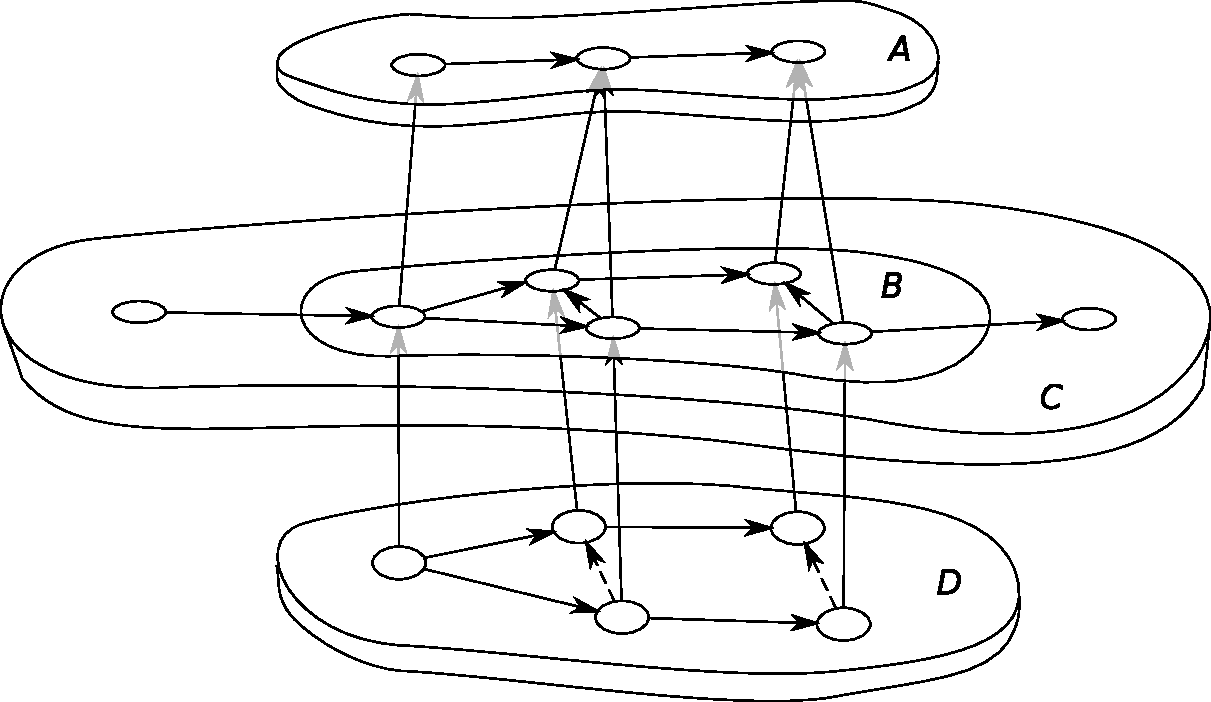
\includegraphics[width=0.7\linewidth]{domain-polysistem}
\caption[Полиситема онтологий предметной области]{\footnotesize Представление предметной области в виде полисистемы онтологий. \\[0.3em] {Слои $A$, $C$ -- стандартные онтологии; $A$, $B$ -- слои, категории; $B$ -- ядро (категория) стандартной онтологии $C$; $B\to A$ -- интерпретация объектов и стрелок $B$ в онтологии $A$ (морфизм); $D$ -- онтология предметной области; $D\to B$ -- интерпретация предметной области $D$ (онтологии, категории, слоя) в слой $B$. Пунктирные стрелки восстановлены в $D$ по их аналогам из $B$. Морфизмы стрелок между слоями на рисунке не отображены.}}

  \label{fig:domain-polysistem}
\end{figure}

Основная цель исследований -- разработка методики рекурсивной декомпозиции автоматизируемой предметной области и ее привязка к существующим слоям полисистемы онтологий. Такая привязка позволяет переносить существующие программные реализации теорий слоев на новые слои по их образу и подобию.

В 2016 году в рамках исследования разработана программная инфраструктура для хранения слоев полисистемы с использованием существующих стандартных онтологий. Слой представляет собой часть онтологии (ядро), которая подвергается отображению в другой слой через функтор или является результатом такого отображения. Слои хранятся в онтологической базе в виде графов. Хранилище онтологий реализовано при помощи системы ClioPatria, использующей язык логического программирования Prolog в качестве языка реализации.  Это позволяет создавать логические теории слоев непосредственно на сервере. Кроме того, декларативная сущность Prolog-а значительно упрощает задачу переноса реализаций теорий между слоями, т.е. порождение программ-аналогов.

В хранилище онтологий загружен ряд онтологий, предназначенных для описания организационной структуры предприятий, сообществ и документов. Разработаны программные модули для представления аннотаций документов в стандарте Open Annotation и NEPOMUK (Network Environment for Personalized, Ontology-based Management of Unified Knowledge), а также данные физических и юридических лиц -- FOAF, в онтологическом хранилище, а также модули для порождения аннотаций из результатов анализа текстов документов.

Разработанная распределенная система применена в решении задачи автоматизации анализа структуры текстов учебных программ технического вуза. Для этого произведена разметка абзацев учебных программ обозначениями концептов, задающих семантическое значение материалу, представленному в абзаце или таблице. Затем выполнено машинное обучение, направленное на распознавание концепта в зависимости от свойств, выделенных в абзаце (наличие ключевых слов, определенных словосочетаний и стилей представления текста). Результатом применения синтезированной системы знаний является семантическая разметка документа, которая отображается на слои полисистемы, что в дальнейшем позволяет применять к элементам документов те или иные алгоритмы обработки данных, а также стили и форматы отображения.

% \end{document}


\section{Проблематика MDE}
\label{sec:problem-mde}

Основная проблема разработки программного обеспечения (ПО) -- это сложность, связанная с большим количеством взаимодействующих гетерогенных компонент в рамках одного программного комплекса.  В основе каждого компонента находится модель, являющаяся продуктом анализа предметной области (см. рис.  \ref{fig:mde-gen-schema}), которая должна изменяться в соответствии с изменением предметной областью.

Качество получаемых программных комплексов (ПК) существенно зависит от надлежащего \emph{целенаправленного} структурирования моделей ПК.~Т.~е.  методологию ТРИЗ\footnote{Теории рационализации и изобретательства.}, весьма широко используемую в строительстве и машиностроении, начали использовать только сейчас при проектировании сложных ПК.~ТРИЗ направляет процесс мышления (arrow thinking) в конструктивном продуктивном направлении. Автоматный подход и подходы на интуитивных уточнениях алгоритма недостаточны для выражения структур и семантики сложных современных систем. Дачные подходы не предоставляют адекватных методов и инструментов для спецификации и описания межструктурных отношений и операций над структурами, что является основой современных подходов к разработке ПО.~В то числе, классическое образование разработчиков, основанное на математике Бурбаки, является причиной скептицизма по отношению применимости современных математических подходов в инженерии ПО.

Процесс внесения изменений в ПО представляет собой исправление программного кода, при этом отображаемая им модель становиться неактуальной.  Основная задача MDE -- это использование интеллекта разработчика на этапе моделирования, а не кодирования. Программный код -- это специальнывй вариант модели ПО, являющийся клнечным шагом последовательного уточнения модели\footnote{Здесь наше понимание процессов преобразования MDA PIM в PSM полностью совпадает.}.

Теорию категорий (ТК) следует рассматривать как общую глобальную теоретическую среду (framework), применимую на всех уровнях моделирования ПО.  Если за основу берется циклическая методика инженерии ПО (Инжерения ПО -> Информатика -> Математика -> Категорная метаматематика -> Инженерия ПО), то ТК помещается в центр модели, и это значительно унифицирует процессы моделирования в инжерении ПО.

\begin{figure}[htbp]
  \centering
  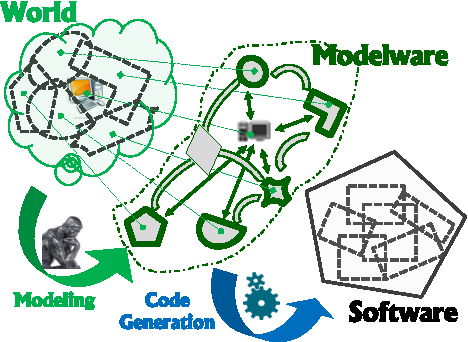
\includegraphics[width=0.5\linewidth]{mde-general}
  \caption{Общая схема MDE}
  \label{fig:mde-gen-schema}
\end{figure}

Система строится из отдельных моделей, которые представляют оригинальный объект.  Объект -- структура целостная, и его компоненты, представленные в виде моделей, перекрывают друг друга, взаимодействуют друг с другом. Класс моделей включает модели в виде структурных объектов отображаемых друг в друга. А это основной феномен категорий -- функтор.

\section{Юниверсум моделей}
\label{sec:mmodcat}

Модели -- это многосортные структуры, являющиеся элементами при построении теории \emph{метамоделей}.  Рассмотрим обобщенный вид такой теории из [39;20].  Метамодельная категория $\mathbfit{M}=(G_M,C_M)$, где $G_M$ -- граф (или более общий вариант a priori заданного предпучка топоса $\mathbfit{G}$), а $C_M$ -- \emph{множество ограничений} (т.е. свойства диаграммы\footnote{Специальная категория, в т.ч. функтор.}), заданных над $G_M$.  \emph{Экземпляром} метамодели $\mathbfit{M}$ является пара $A = (G_A, t_A)$, где $G_A$ -- это другой граф (объект в $\mathbfit{G}$) и $t_A: G_A \to G_M$ -- отображение (стрелка в $\mathbfit{G}$), которую следует понимать как \emph{определение типа}, которые удовлетворяют ограничению $A \models C_M$ (более детально в [20]).  \emph{Отображение экземпляров} $A\to B$ -- это отображение графов $f: G_A\to G_B$, которое совместно с определением типа $f;t_B = t_A$ дает коммутативную диаграмму.  Эти элементы задают категорию $\mathbfit{Mod}(M) \subset \mathbfit{G}/G_M$ $M$-экземпляров.

Чтобы как-то объединить в одну структуру разрозненные гетерогенные экземпляры различных метамоделей, определим метамодельные морфизмы $m: M\to N$ как [sketch]-морфизмы, т.е., отображения графов $m: G_M\to G_N$ совместимые по ограничениям.  Эти отображения задают категорию $\mathbfit{MMod}$.  Теперь можно объединить все категории $\mathbfit{Mod}(M)$ в одну категорию $\mathbfit{Mod}$, где объектами являются экземпляры (= G-стрелки\footnote{Есть категории стрелок, но, вроде, не данный случай.}) $t_A: G_A\to G_{M(A)}$, $t_B: G_B\to G_{M(B)}$ и т.д., причем каждая стрелка имеет свою метамодель, а морфизмы $f:A\to B$ являются парами $f_{data}: G_A\to G_B$, $f_{meta}: M(A) \to M(B)$ такие, что $f_{data};t_B = t_A; f_{meta}$, т.е., образуют коммутативные квадраты в $\mathbfit{G}$.  Таким образом, $\mathbfit{Mod}$ -- это подкатегория категории стрелки $\mathbfit{G}^{\to}$.

Можно показать, что [[ко]предельный] декартов квадрат (коамальгама), построенный на действительном экземпляре $t_B: G_B\to G_N$ метамодели $N$ вдоль [sketch]-морфизма $m:M\to N$ приводит к действительному экземпляру $M$ [20].  Таким образом определяется расслоение $\mathbfit{p} : \mathbfit{Mod} \to \mathbfit{MMod}$, чей декартов подъем порождается этими предельными декартовыми квадратами.

\section{Трансформация моделей (MDA)}
\label{sec:mda-transform}

По большому счету MDE не интересует процесс трансформации в программный код, т.~к. интересует больше процесс внесения изменений (актуализация категории метамодели). Но в целом трансформация представляет собой последовательное уточнение описания модели до конкретных модулей, реализованных в конкретной среде программирования.

\section{Подходы к внесению изменений в модели}
\label{sec:mde-conversions}

В настоящее время выделяются два подхода к реализации трансформации -- \emph{физическое объединение моделей} и \emph{распространение изменений}.  В первом подходе последовательно на каждом этапе объединения из двух моделей строится одна, при этом общие концепты сливаются в один.  Второй подход базируются на расслоении категории метамоделей на отдельные модели, связанные друг с другом через функторы.  Эти функторы в нотации полисистемного анализа и синтеза реализуют интерпретации объектов и стрелок (морфизмов).

Процесс объединения моделей (первый случай) состоит из двух шагов -- а) создание спецификации объединения, и этот этап является творческим, б) собственно объединение, представляющее собой выполнение алгебраических операций над моделями с целью построить общий копредел диаграммы (категорию) (см. рис.~\ref{fig:amalgama}).  Случай аналогичный этому рассматривается в диссертации д.ф.--м.н. Ковалева Сергея (ИДСТУ СО РАН выступал в качестве ведущей организации в 2012 году).  Основное достоинство подхода, основанного на объединении моделей, -- это первый шаг в трансформации: в результате объединения создается модель модуля, где все функции интегрированы в модуль, что влечет более оптимизированный программный код (далекий от MDE пример -- LLVM).  У С. Ковалева в качестве базовой методики проектирования выступало аспект-ориентированное программирование, где исходными моделями для трансформации служили амальгамы (копределы) таких объединений.  Из диссертации не понятно было как они строились на практике, были изучены их свойства.

\begin{figure}[htbp]
  \centering
  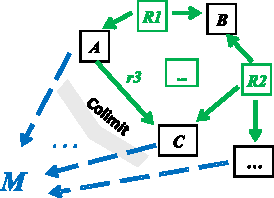
\includegraphics[width=0.5\linewidth]{amalgama}
  \caption{Построение амальгамы в процессе объединения моделей\\[0.3em]
    \protect\footnotesize{$M$--требуемая объединенная модель, $A,B,C\ldots$ -- исходные модели.}}
  \label{fig:amalgama}
\end{figure}

Во втором случае трансформация моделей представляет собой процесс восстановление сквозной интерпретации концептов и стрелок в расслоении, в случае, если одна из моделей (слой) подверглась изменению.  Актуализация представляет собой преобразование пары морфизмов (межслойная интерпретация; измененная структура в слое, рис.~\ref{fig:propagation}) в новую пару морфизмов и распространение этой процедуры на другие слои.  Достоинство подхода -- более естественное для человека представление метамодельной категории (в виде слоев) и локализованная процедура изменений (не зтрагивается все модель в целом).


\begin{figure}[htbp]
  \centering
  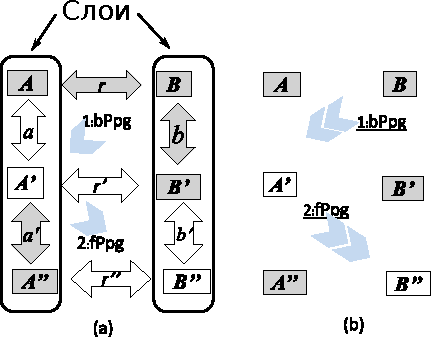
\includegraphics[width=0.5\linewidth]{propagation}
  \caption{Распространение изменений\\[0.3em]
    \footnotesize{Закрашенные фигуры -- состояние полисистемы до запуска
      процесса распространения изменений, незакрашенные -- результат процесса.
      $A',B',r'$ и т.п. -- производные объекты и отображения; $bPpg$ --
      ``обратное'' распространение изменения (морфизм $(r,b)\to (a,r')$), $fPpg$
      -- прямое ($(r',a')\to (r'',b')$).  В случае (b) перед распространением
      еще вычисляются отношения между объектами, в (a) они заданы.}}
  \label{fig:propagation}
\end{figure}


В обоих случаях присутствуют этапы, где необходимо задействовать творческий потенциал разработчика.  В первом случае -- формирование спецификации объединения, во втором -- изъятие недостающей информации при актуализации эпиморфизмов и мономорфизмов.  Во втором случае имеет смысл исследовать возможности компьютера в самообучении: строить слои моделей (UML, Онтологических, Реляционных и т.п.) по мере поступления информации от пользователя и проведения актуализации на предыдущих циклах разработки.  Чем больше структур удастся ассимилировать, тем меньше вопросов надо будет задавать разработчику.

\section{Построение метамодельной категории}
\label{sec:mmod-construction}

На первоначальном этапе MDE существует проблема первоначального построения метамодельной категории, т.е. для построения полной системы (категории) моделей необходимо выделить в предметной области объекты и модели и построить функторы между концептами и моделями, т.е. объекты категории метамодели $\mathbfit{MMod}$ и морфизмы в этой категории.  В качестве методики предлагается использовать методологию полисистемного анализа и синтеза, а метамодель строить как полисистему.  В какой-то мере она отражена рис.~\ref{fig:propagation}b.

Разработанные процедуры распознавания концептов на примере рабочих и учебных программ вуза -- это примеры реализации этой задачи.  По набору примеров (абзацев), их характеристических свойств (морфизмы модели), определяется концепт (название сущности, свойства), связь между концептами и свойствами, а также между концептами, в нашем случае -- это описания, последовательности и зависимости (структурные и семантические), затем, задаются отображения этих элементов в другие слои (например, мереологический, автоматный, логический и т.д.).  В качестве трансформации выступает процедура представление системы модулей, всяческие проверки на полноту (относительно требуемых в слоях отношений между известными/распознанными концептами), генерация новых версий представлений (по новым ФОС) и т.п.

\section{К решению задачи разработки методики построения онтологической модели предметной области}
\label{sec:technique-onto}

Здесь необходимо доделать задачу анализа процесса разработки программы, фиксируемого в репозитариях типа GIT\@.  Задача состоит в том, чтобы в сообщениях программистов выделить концепты и построит в слоях семантическую интерпретацию через указание кусков кода, реализующих интерпретацию этого концепта. Для решения этой задачи пригодится весь собранный и сконструированный инструментарий обработки естественно-языковых текстов.

Полученные к настоящему моменту результаты (задел) опубликованы в докладе \href{http://mipro-proceedings.com/sites/mipro-proceedings.com/files/upload/cis/cis_025.pdf}{Extraction of Thesaurus and Project Structure from Linux Kernel Source Tree}.

\section{Развернутый научный отчет РФФИ 00166\\Технология интеграции распределенных web-сервисов и данных в рамках междисциплинарной информационно-аналитической среды}
\label{sec:RFBRReport}

\begin{quote}
В настоящее время активно развиваются \textbf{научные исследования окружающей среды} и управления природно-ресурсным потенциалом, \textbf{носящих междисциплинарный характер} и требующих \textbf{интеграции и комплексного использования методов обработки научных пространственных ресурсов}. Увеличение скорости передачи данных сети Интернет, развитие и стандартизация программного интерфейса браузеров позволяют \textbf{удаленно использовать методы в виде сервисов} на основе стандартов Open Geospatial Consortium (OGC), которые обеспечивают взаимодействие различных программных систем через Интернет. Это обуславливает актуальность комплексного использования распределенных разнородных сервисов и данных, для которых требуются новые подходы к представлению пространственных данных, передачи пространственных данных между сервисами, поиску сервисов, согласованию форматов данных, организации асинхронного вычислительного процесса, где операторами являются сервисы и т.д. В рамках проекта планируется создание технологий разработки Web Processing Service (WPS) сервисов на основе\textbf{ библиотек программного кода}, языков сценариев, методов доступа к базовым пространственным данным и другого ПО, повышающих эффективность разработки, объединения и использования разных сервисов для \textbf{проведения междисциплинарных исследований окружающей среды региона и управления его природно-ресурсным потенциалом}.

(2016)
\begin{enumerate}
\item Разработать сервис классификации GRID данных на основе правил пользователя. Разработать методы применения SLD стилей для результатов работы сервисов на основе расширения набора метаданных сервисов. Создать механизм передачи сервисам результатов запроса к табличным данным, для что позволит перед запуском сервисов выполнять их фильтрацию и обобщение данных . Исполнители: Бычков И.В., Фёдоров Р.К., Ружников Г.М.

\item Разработать Web-приложения конвертирования неструктурированной информации, представленной в формате табличного процессора, в базы данных, на основе логического вывода правил анализа табличной компоновки. Развить методы словообразования в совокупности с методами фонетического и орфографического анализа для повышения качества очистки данных и приведения к эталонным значениям в процессе интеграции разнородных табличных документов. Повысить качество очистки данных на основе их структурного описания. Исполнители: Бычков И.В., Шигаров А.О., Парамонов В.В.

\item Разработать сервисы конвертации в формат SMD для геоданных, представленных в PostGIS. Разработать сервисы построения файлов MRG по пользовательским данным. Исполнители: Хмельнов А.Е., Фереферов Е.С., Гаченко А.С.

\item Моделирование сервисов на основе онтологического подхода (2014). Создание подсистемы индуктивного приобретения знаний о предметной области на основе анализа изменений структур данных компонент программ (информационно-вычислительного ресурса). Разработать технологию построения моделей информационных потоков в вычислительных сетях на основе анализа изменений их структуры (2016). Исполнитель: Е.А. Черкашин
\end{enumerate}
\end{quote}

\subsection{Степень достижения поставленных в проекте целей}
 (2014)На основе онтологического подхода разработаны структурные спецификации
 параметров WPS-сервисов, которые позволяют определить требования к параметрам в
 виде реляционных таблиц.
 (2015)

 \subsection{Степень новизны полученных результатов}
 (2014) Впервые на основе онтологического подхода параметры WPS-сервисов могут быть специфицированы, что позволяет автоматизировать поиск данных определенной структуры с определенными типами и единицами измерений, конвертацию данных и формирование пользовательского интерфейса для ввода данных. (2015)



\subsection{Полученные в ходе выполнения Проекта важнейшие результаты}
(2014) <<нет>>

(2015) Предложена технология построения вопросно-ответных диалоговых подсистем, ориентированных на приобретение информации от пользователя, базирующаяся на полисистемном онтологическом представлении предметной области информационного ресурса.

(2016) Развит подход к полисистемному онтологическому моделированию предметной области информационных систем.  Подход применим для решения задач формализации спецификаций реляционных данных как параметров WPS, ведения диалога с пользователем, в частности построения запросов на естественном языке, ведения диалога с пользователем.

\subsection{Сопоставление полученных результатов с мировым уровнем}
(2015) Разработанный подход к построению вопросно-ответных подсистем развивают современные подходы как в теоретическом и в прикладном аспектах: процедуры вывода сценария диалога представлены в виде полисистемы - структуры объединяющей различные аспекты модели предметной области через морфизмы слоев. Предложен подход к представлению знаний системы при помощи технологий Семантического Веба - одного из основных направлений исследований в области сетевого взаимодействия приложений. Представленный подход к формированию сценария диалога является оригинальным, т.к. использует специальную методологию системного анализа (процедуру полисистемного расслоения, которая ранее в таких задачах не была использована).

(2016) ? Надо ли в этом году это писать. ?

\subsection{Методы и подходы, использованные в ходе выполнения Проекта (описать,
  уделив особое внимание степени оригинальности и новизны)}

(2016) Предметная область информационной системы представляется в виде полисистемы онтологий. Полисистема онтологий - это расслоенная структура, где каждый слой в идеале представляет собой категорию; элементы категории отображаются в элементы других слоев (концепты в концепты, стрелки в стрелки), и такое отображение, функтор, есть интерпретация одного слоя другим. Интерпретация позволяет переносить алгоритмы и программы, реализующие свойства одного слоя, в другой, строить процедуры обработки данных по образу и подобию, а также обеспечивать верификацию слоев на структурную корректность и полноту, строя указанные интерпретации.

Полисистема онтологий строиться из существующих стандартных онтологий, например, разработанных в проекте Linked Data. Слой строится из той части онтологии, которая представима в виде полноценной категории, затем требуется построить интерпретацию в другой слой, такую, чтобы все концепты и стрелки нового слоя были отображены в другой слой.

Полисистемное представление онтологий позволяет полностью использовать все наработанные с 2001 года технологии Семантического Веба, а также обобщить большинство расширений семантическох сетей, например, самой известной -- MultiNet (MeshNet, \url{http://pi7.fernuni-hagen.de/forschung/multinet/multinet_en.html}).

Для представления в виде полисистемы онтологий предметной области разрабатываемой информационной системы адаптирована методика полисистемного расслоения (Черкашин А.К.,1997)), которая ранее в таких задачах не была использована. При этом система концептов строится, например, в результате автоматизированного анализа текста входных документов существующими методами. В результате такого анализа должны быть выделены ключевые слова, построена иерархическая классификация входных документов по схожести друг с другом и выделены ключевые термины, характеризующие основные узлы классификации. Эти термины задают тезаурус, разновидность онтологии, где концепты связаны друг с другом отношением ``is-a''.  Затем эти концепты должны быть привязаны через интерпретацию к слою полисистемы онтологии, который лучше всего соответствует тезаурусу. Если такой слой существует, то на следующем шаге тезаурус дополняется отношениями, имеющими интерпретацию в смежном слое полисистемы, т.к. все слои должны быть связаны морфизмами.

На этапе дополнения тезауруса предложен вариант методики ведения диалога с пользователем, цель которого дополнить структуру разрабатываемой концептуальной модели задачи до выполнения свойства полноты относительно структуры смежных слоев. Вопросы диалога синтезируются на основе анализа структуры морфизма и стрелок в смежных слоях. В диалоге ответ, название отношения, можно выбирать из возможных вариантов существующих отношений (стрелок) в слоях или задавать новые имена, если ничего подходящего в полисистеме нет.

{\bfseries Другой задачей, решаемой при помощи полисистемного подхода является анализ изменения структуры семантически размеченных документов и построения модели информационных потоков. Информационный поток представляется в виде преобразования ... Два документа должны содержать общую логическую структуру (ссылку на один и тот же объект), а документы должны относится к разным классам.... Документ логически связывает структуры, и данная связь интерпретируется как преобразование исходной структуры в ряд новых. (В конечном счете хотим получить устойчивые паттерны преобразований объектов)
}

С использованием технологий Семантического Веба разработана спецификация параметров WPS-сервисов, которые позволяют определить требования к параметрам в виде реляционных таблиц.  Спецификация определяет название параметра (сущности) и набор атрибутов. Каждый атрибут характеризуется названием, именем в базе данных, типом данных, единицами измерения (для числовых данных), элементом управления и его свойствами. Элемент управления определяет для атрибута пользовательский интерфейс редактирования и отображения данных. Свойства элемента управления позволяют настраивать пользовательский интерфейс в зависимости от характеристик данных, например, единицы измерения для числовых данных или определять тип географических данных. Спецификации представлены в виде каталога. Применение спецификаций позволяет настраивать WPS-сервис на структуру и свойства данных пользователя, в том числе
\begin{enumerate}
\item Создавать таблицы, требуемые для определенного сервиса анализа или обработки данных, на основе спецификаций параметров.
\item Обобщать различные по структуре пользовательские таблицы, содержащие общую спецификацию или унаследованные от нее другие спецификации.
\item Применять WPS-сервисы к любым таблицам содержащими данную спецификацию или спецификацию, унаследованную от данной.
\item Проводить анализ и создавать отчеты по совмещенным пользовательским таблицам.
\end{enumerate}

Дальнейшая разработка данной технологии позволит существенно продвинутся в решении задач адаптации/конвертации данных документальных источников (таблиц, отчетов) к структуре входных данных сервисов WPS, разрабатывать алгоритмы интерпретации результатов расчетов в виде документов, предназначенных для чтения пользователем, а также интегрировать WPS в системы документооборота.

% Приложения разработанных WPS
{\bfseries
В рамках проекта разработаны алгоритмы и программная реализация нескольких методик анализа структуры (пластики) рельефа на основе ГРИД-данных высот. Программное обеспечение позволяет выделять в структуре рельефа местности зоны конвергенции и дивергенции вещества, а также проводить автоматизированный анализ объемов ... Алгоритмы и программное обеспечение использовано в исследованиях разломной микроструктуры рельефа Западного побережья оз.~Байкал в Ольхонском районе Иркутской области. Алгоритмы строятся на основе матричного преобразования поля градиентов высоты рельефа, а также фильтрации координат точек ГРИДА на основе логических ограничений с последующей аппроксимацией поверхностей трехмерными сплайнами.
}

\subsection{Вклад каждого члена коллектива в выполнение Проекта в 2016 году
  (указать работу, выполненную каждым членом коллектива по Проекту в 2016 году с
  новой строки)}
(2015) Методика и программное обеспечение индуктивного приобретения знаний о предметной области, основывающаяся на анализе изменений структур данных компонент программ и поддержки диалога с пользователем/разработчиком информационно-вычислительного ресурса (Черкашин Е.А.).

(2016) ...


\subsection{Адреса (полностью) ресурсов в Интернете, подготовленных авторами по
  данному проекту, например, http://www.somewhere.ru/mypub.html}

\url{https://github.com/CellulaProject};\\
\url{https://github.com/eugeneai/python-pengines};\\
\url{https://github.com/eugeneai/ontology-server};\\
\url{https://github.com/eugeneai/dockerfiles/tree/master/ontology-server};\\
\url{https://github.com/eugeneai/dustjs}.

\begin{thebibliography}{9}
\bibitem{CTMDE} Zinovy Diskin, Tom Maibaum. \emph{Category Theory and
    Model-Driven Engineering: From Formal Semantics to Design Patterns and Beyond}. Proceedings of ACCAT 2012
EPTCS 93, U. Golas, T. Soboll (Eds.), 2012, pp. 1–21, doi:10.4204/EPTCS.93.1. URL:\url{http://arxiv.org/pdf/1209.1433.pdf}.
\end{thebibliography}

% \section{Библиотека категорий, использованных в статье}
% \label{sec:catlib}

% Пусть $\mathbfit{C}$ -- категория, тогда $\mathbfit{C}^\to$ -- категория
% стрелок, состоящая из объектов $f: X\to Y$ (объектами являются морфизмы),
% морфизмов -- коммутативных квадратов
% \begin{figure}[h]
%   \centering
%   \begin{tikzpicture}
%     \node (X) {$X$};
%     \node (Y) [right of=X] {$Y$};
%     \node (Xp) [below of=X] {$X'$};
%     \node (Yp) [right of=Xp] {$Y'$};

%     \draw[->] (X) to node {$\small f$} (Y);
%     \draw[->] (Xp) to node {$\small f'$} (Yp);
%     \draw[->] (X) to node {$\small m$} (Xp);
%     \draw[->] (Y) to node {$\small n$} (Yp);
%   \end{tikzpicture}
% \end{figure}

% \noindent{}При этом $X,Y,X',Y'\in Ob(C)$, и $f,f',n,m \in Hom(C)$ ввиду того, что $n\circ
% f=f'\circ m$ (диаграмма коммутативна).

\end{document}


%%% Local Variables:
%%% TeX-master: t
%%% End:
